\documentclass[border=8pt]{standalone}
\usepackage[T1]{fontenc}\usepackage[utf8]{inputenc}\usepackage{lmodern}
\usepackage{tikz}\usetikzlibrary{arrows.meta,positioning}
\begin{document}
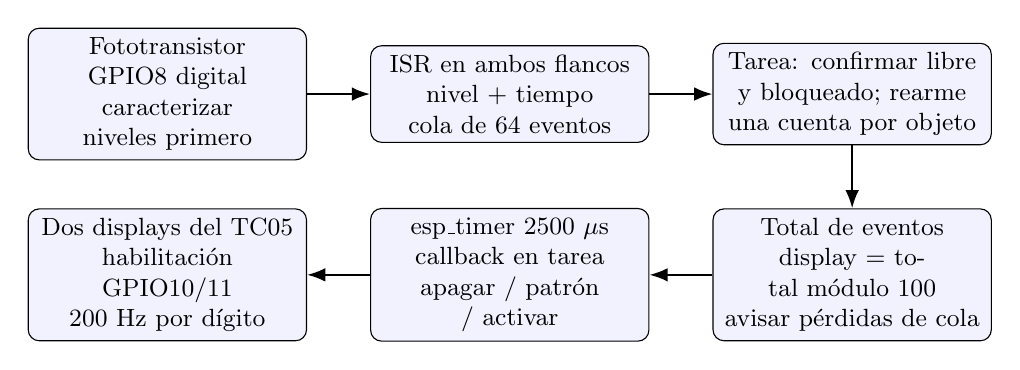
\begin{tikzpicture}[>=Latex,font=\small,node distance=0.8cm,
 b/.style={draw,rounded corners,fill=blue!5,text width=3.3cm,align=center,minimum height=1.2cm}]
\node[b] (sensor) {Fototransistor\\GPIO8 digital\\caracterizar niveles primero};
\node[b,right=of sensor] (isr) {ISR en ambos flancos\\nivel + tiempo\\cola de 64 eventos};
\node[b,right=of isr] (task) {Tarea: confirmar libre\\y bloqueado; rearme\\una cuenta por objeto};
\node[b,below=of task] (data) {Total de eventos\\display = total módulo 100\\avisar pérdidas de cola};
\node[b,left=of data] (timer) {esp\_timer 2500 $\mu$s\\callback en tarea\\apagar / patrón / activar};
\node[b,left=of timer] (disp) {Dos displays del TC05\\habilitación GPIO10/11\\200 Hz por dígito};
\draw[->,thick] (sensor)--(isr);\draw[->,thick] (isr)--(task);\draw[->,thick] (task)--(data);
\draw[->,thick] (data)--(timer);\draw[->,thick] (timer)--(disp);
\end{tikzpicture}
\end{document}
